\section{Результаты решения задачи и их анализ}

Для задача была решена с различными значениями максимально допустимой относительной погрешности на шаге решения задачи Коши для $\Delta = 10^{-7}, 10^{-9}, 10^{-11}.$ При каждом проходе были посчитаны погрешности на шаге (по правилу Рунге см. выше), а так же глобальные погрешности, а именно $\mathrm{Err} = 6.82\cdot 10^{-07}$.\\

Для сравнения численного решения и аналитического можно взглянуть на полученные графики, по которым явно видно, что они абсолютно идентичны.

\begin{figure}[H]
\noindent\centering{
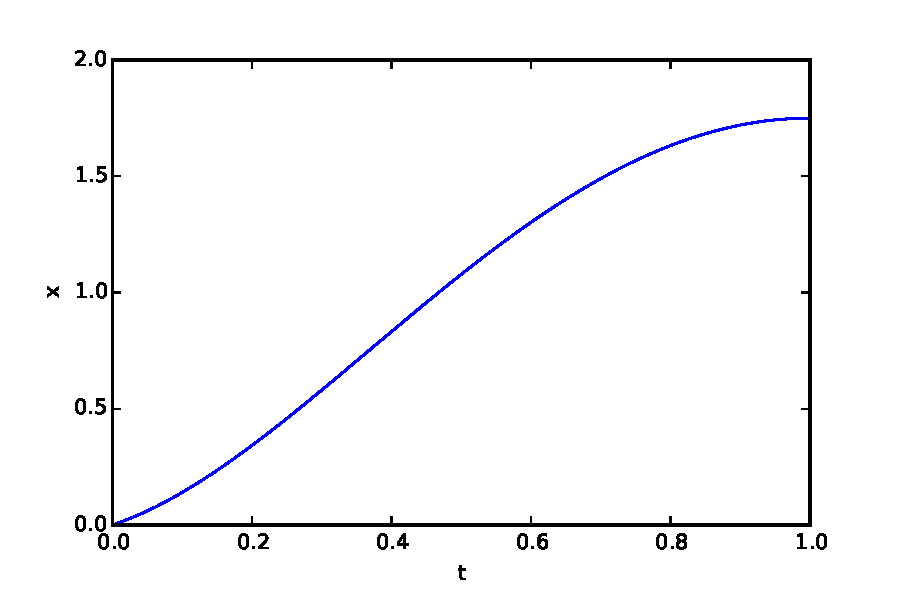
\includegraphics[width=110mm]{pictures/01t-x.pdf} 
  \caption{График зависимости $x(t)$, полученный численным методом.}}
\end{figure}
\begin{figure}[H]
\noindent\centering{
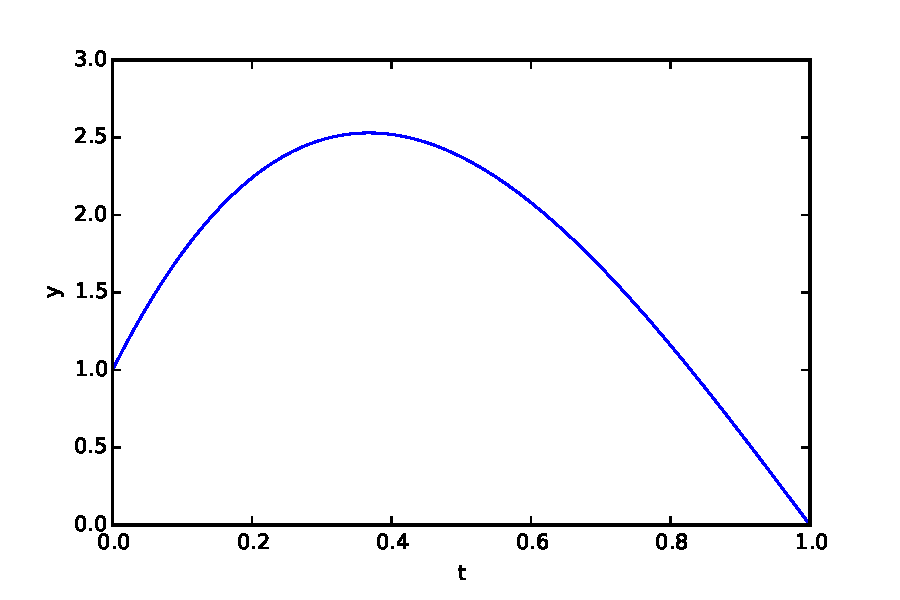
\includegraphics[width=110mm]{pictures/01t-y.pdf} 
  \caption{График зависимости $y(t)$, полученный численным методом.}}
\end{figure}
\begin{figure}[H]
\noindent\centering{
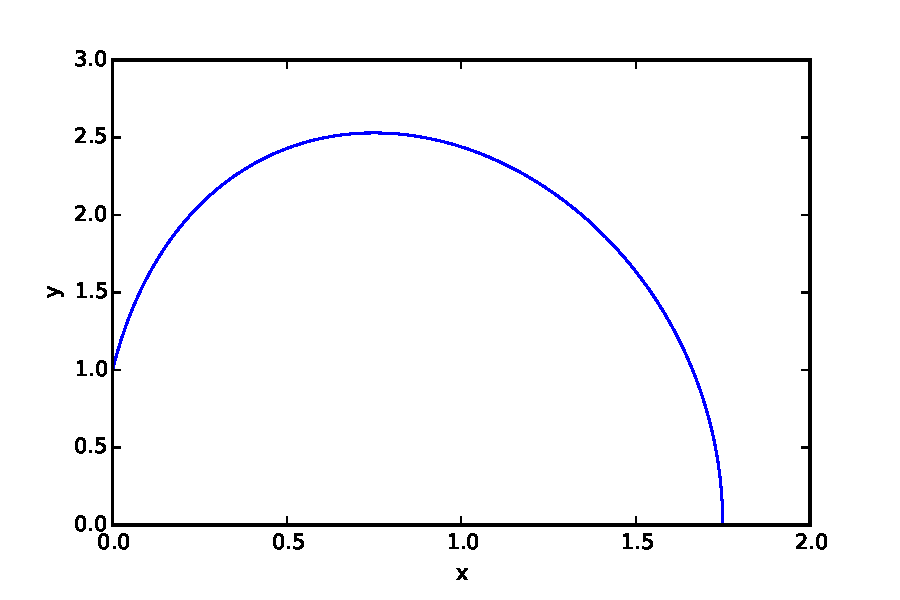
\includegraphics[width=110mm]{pictures/01x-y.pdf} 
  \caption{График зависимости $y(x)$, полученный численным методом.}}
\end{figure}
\begin{figure}[H]
\noindent\centering{
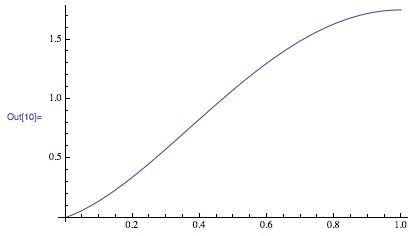
\includegraphics[width=110mm]{pictures/xt.png} 
  \caption{График зависимости $x(t)$, полученный аналитичсеки.}}
\end{figure}
\begin{figure}[H]
\noindent\centering{
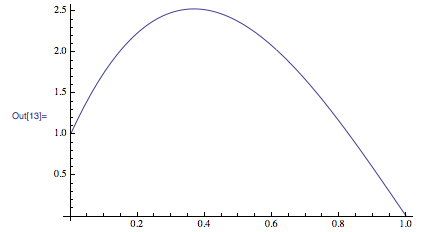
\includegraphics[width=110mm]{pictures/yt.png} 
  \caption{График зависимости $y(t)$, полученный аналитичсеки.}}
\end{figure}
\begin{figure}[H]
\noindent\centering{
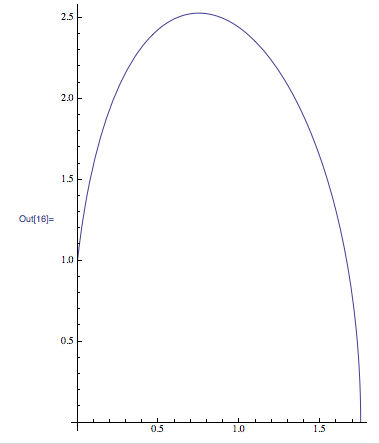
\includegraphics[width=110mm]{pictures/xy.png} 
  \caption{График зависимости $y(x)$, полученный аналитичсеки.}}
\end{figure}